% -*- compile-command: "pdflatex report.tex"; -*-
\documentclass[a4paper,12pt]{article}
\usepackage[utf8]{inputenc}
\usepackage[english]{babel}
\usepackage{graphicx}
\usepackage{listings}
\usepackage{hyperref}
\lstset{
language=C,
basicstyle=\footnotesize
}

\title{Let it snow}
\author{Christian Luckey}
\author{Matteus Hemström}

\begin{document}

\maketitle

\newpage

\section{Introduction}

We set out with one simple task: We wanted to make it snow with real time graphics. We wanted to create a real time world looking like Figure~\ref{fig:youtube}:

\begin{figure}[ht]
  \centering
  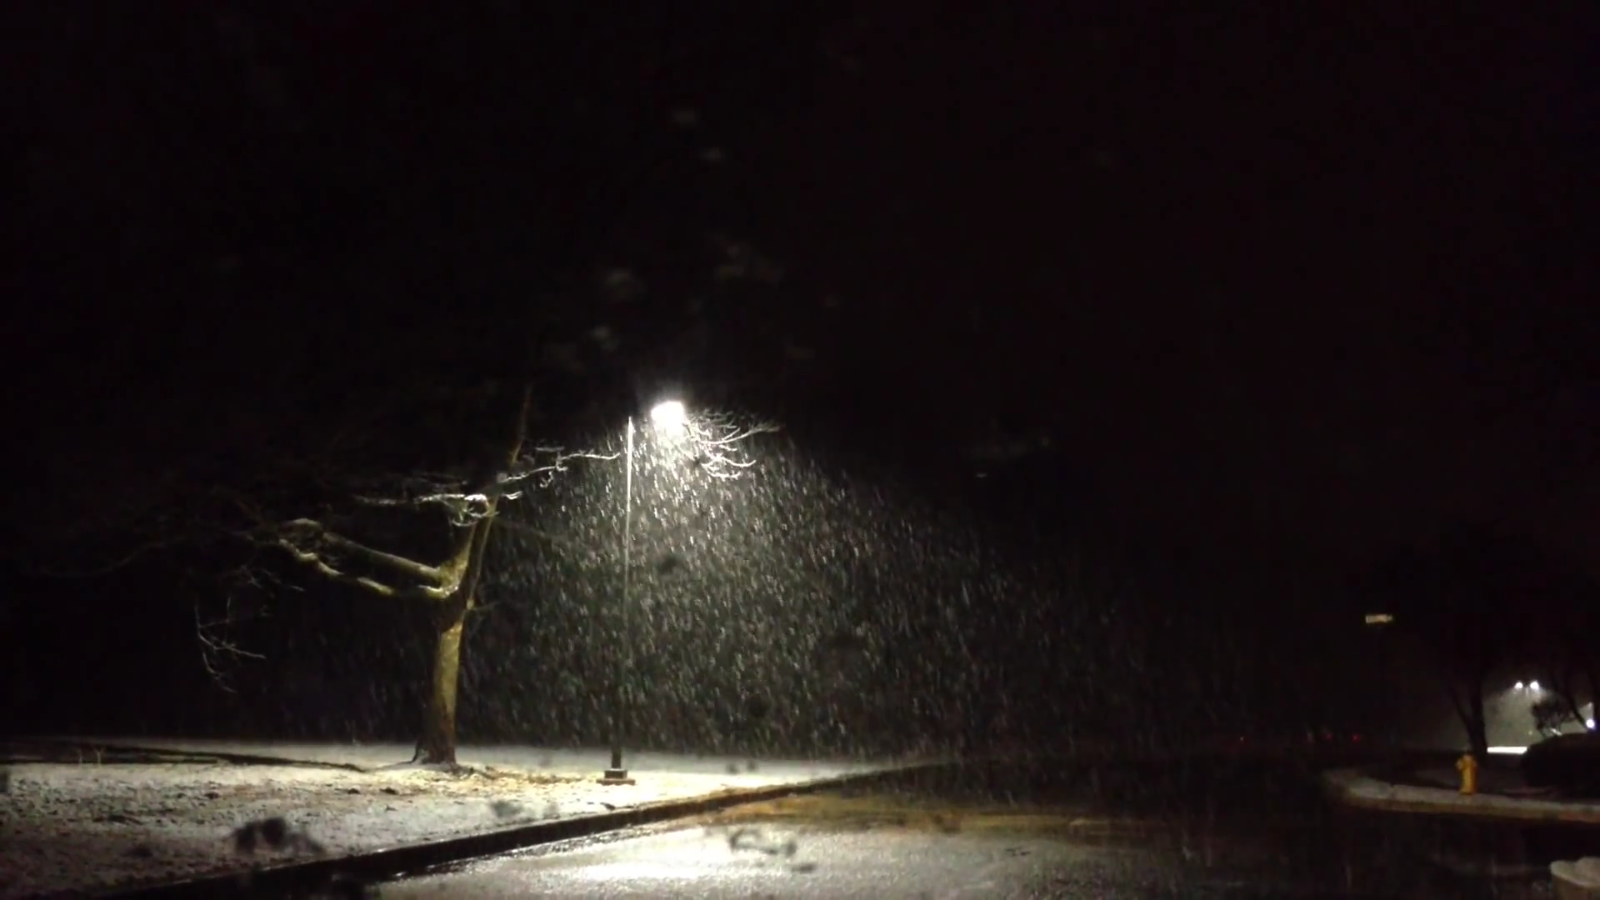
\includegraphics[width=0.9\textwidth]{youtube}
  \caption{\label{fig:youtube} Source: \href{https://www.youtube.com/watch?v=vHZb2xdVTCA}{https://www.youtube.com/watch?v=vHZb2xdVTCA}}
\end{figure}
\noindent
And off we went!



\section{Background}

In Figure~\ref{fig:youtube} and associated video we can identify a couple of elements being present:

\begin{enumerate}
  \item Models for trees and light posts.
  \item Multiple directed light cones.
  \item Snow on the ground.
  \item Snow tumbling through the air.
  \item Shadows cast on the ground.
  \item Snow stuck and falling on the camera lens.
  \item The camera shaking.
\end{enumerate}

All these has some crux, even the most simplest tasks like placing millions of little snow flakes on the screen. Lets look at them in order.


\subsection{Multiple directed light cones}

We looked into a couple of different techniques when it came to making the light:


\subsection{Snow on the ground}

There were some pretty sophisticated models used in the Disney film Frozen \href{https://disney-animation.s3.amazonaws.com/uploads/production/publication_asset/94/asset/SSCTS13_2.pdf}{[1]}, but we deemed them unfit for real time usage. Then again the reference image has no moving ground snow.


\subsection{Shadows}


\subsubsection{Shadow stensils}

\subsubsection{Shadow Maps}



\subsection{Falling snow}

\subsubsection{Navier Stokes}

In order to simulate the effect of gusts of wind blowing on the snow navier stokes equations could be used \href{http://www.intpowertechcorp.com/GDC03.pdf}{[2]}. The linked paper is about fluid dynamics but since they're pretty much the same we're sure the methods described could still be applied.




\section{Implementation}

\begin{lstlisting}
mat4 model_matrixes[count * count * count];
for (int x = 0; x < count; x++) {
  for (int y = 0; y < count; y++) {
    for (int z = 0; z < count; z++) {
      int pos = x + y * count + z * count * count;
      model_matrixes[pos] = Mult(Mult(T(x * 2, y * 2, z * 2),
          transEverything), Rx(time));
      model_matrixes[pos] = Transpose(model_matrixes[pos]);
    }
  }
}
glBufferData(GL_ARRAY_BUFFER, sizeof(model_matrixes),
    &model_matrixes, GL_STATIC_DRAW);
\end{lstlisting}


\section{Problems}

A lot, like you have no idea how many problems we had.

\subsection{Detangling global state}

We've probably refactored the codebase completelely somewhere around three times, trying to untangle it from iself.

\subsection{Shadow buffer bugs}

We ended up wasting about a week trying to debug a fully working implementation of shadow maps, only that it didn't render correct on the specific hardware we were developing it on.

\section{Conclusions}

What we got was this:


\end{document}